\documentclass{article}

\usepackage{graphicx}
\usepackage{hyperref}

\title{User Interface Parsing \\ \small{Progress Update}}
\author{Calvin Loncaric}
\date{May 13, 2015}

\begin{document}

\maketitle

\noindent Since the last update I have been working on high-level object
recognition. Since the last update I have written code to:
\begin{itemize}
\item identify how many boxes are likely to exist in the scene,
\item identify those boxes, and
\item identify measurement lines and relate them to the boxes.
\end{itemize}

\noindent My immediate next steps are:
\begin{itemize}
\item improve text recognition accurracy and
\item implement code generation from boxes and measurements to HTML.
\end{itemize}

\begin{figure}
    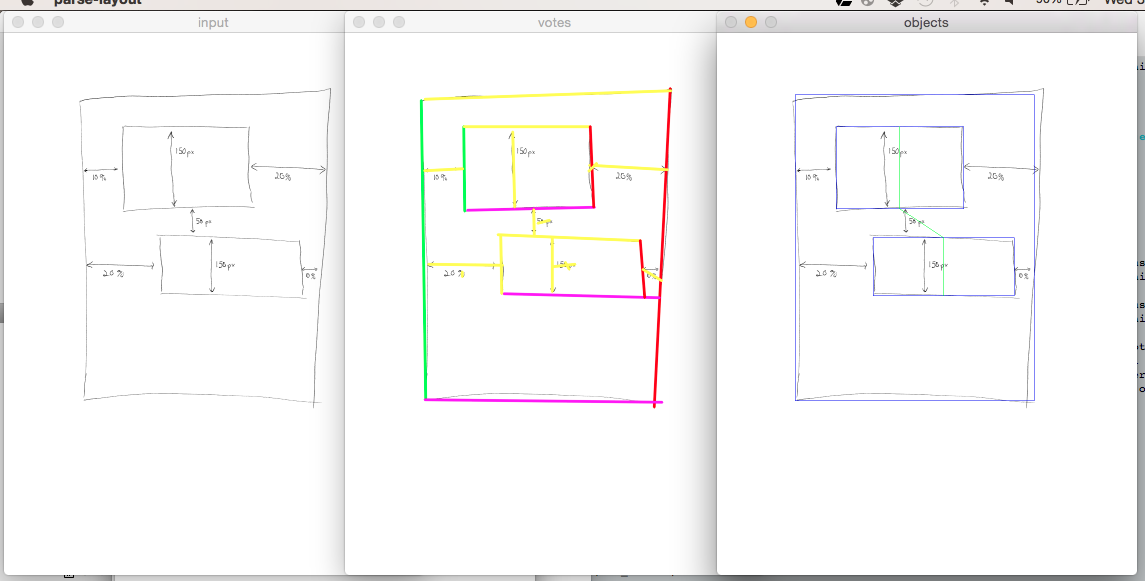
\includegraphics[width=\textwidth]{progress-2015-05-13-screenshot.png}
    \caption{Object identification. The left image is the input. The middle
        image shows stroke classification (each stroke gets multiple
        classifications, which aren't visualized). The right image shows the
        identified objects. (Note that code to identify horizontal measurement
        lines exists and works, but was commented out for this screenshot.)}
    \label{fig:screenshot}
\end{figure}

\end{document}
